\let\negmedspace\undefined
\let\negthickspace\undefined
\documentclass[journal]{IEEEtran}
\usepackage[a5paper, margin=10mm, onecolumn]{geometry}
%\usepackage{lmodern} % Ensure lmodern is loaded for pdflatex
\usepackage{tfrupee} % Include tfrupee package

\setlength{\headheight}{1cm} % Set the height of the header box
\setlength{\headsep}{0mm}     % Set the distance between the header box and the top of the text

\usepackage{gvv-book}
\usepackage{gvv}
\usepackage{cite}
\usepackage{amsmath,amssymb,amsfonts,amsthm}
\usepackage{algorithmic}
\usepackage{graphicx}
\usepackage{textcomp}
\usepackage{xcolor}
\usepackage{txfonts}
\usepackage{listings}
\usepackage{enumitem}
\usepackage{mathtools}
\usepackage{gensymb}
\usepackage{comment}
\usepackage[breaklinks=true]{hyperref}
\usepackage{tkz-euclide} 
\usepackage{listings}
% \usepackage{gvv}                                        
\def\inputGnumericTable{}                                 
\usepackage[latin1]{inputenc}                                
\usepackage{color}                                            
\usepackage{array}                                            
\usepackage{longtable}                                       
\usepackage{calc}                                             
\usepackage{multirow}                                         
\usepackage{hhline}                                           
\usepackage{ifthen}                                           
\usepackage{lscape}
\usepackage{circuitikz}
\tikzstyle{block} = [rectangle, draw, fill=blue!20, 
    text width=4em, text centered, rounded corners, minimum height=3em]
\tikzstyle{sum} = [draw, fill=blue!10, circle, minimum size=1cm, node distance=1.5cm]
\tikzstyle{input} = [coordinate]
\tikzstyle{output} = [coordinate]


\begin{document}

\bibliographystyle{IEEEtran}
\vspace{3cm}

\title{2.7.29}
\author{EE25BTECH11017 - Mahesh Chollangi}
\maketitle
% \newpage
% \bigskip
{\let\newpage\relax\maketitle}

\renewcommand{\thefigure}{\theenumi}
\renewcommand{\thetable}{\theenumi}
\setlength{\intextsep}{10pt} % Space between text and floats


\numberwithin{equation}{enumi}
\numberwithin{figure}{enumi}
\renewcommand{\thetable}{\theenumi}

\textbf{Question}:\\
The area of a triangle formed by vertices $\vec{O}, \vec{A}$ and $\vec{B}$, where $\vec{OA} = \hat{i} + 2\hat{j} + 3\hat{k}$ and $\vec{OB} = -3\hat{i} - 2\hat{j} + \hat{k}$ is


\section*{Solution}

Let \vec{O} be the origin

Represent the vectors in matrix form:
\begin{align}
\vec{A} = \myvec{1 \\ 2 \\ 3}, \quad
\vec{B} = \myvec{-3 \\ 1 \\ 1}
\end{align}

The area of triangle $OAB$ is given by:
\begin{align}
\text{Area} = \frac{1}{2} \norm{\vec{A} \times \vec{B}}
\end{align}

Compute the cross product using determinant:
\begin{align}
\vec{A} \times \vec{B} =
\myvec{
(2)(1) - (3)(1) \\
(3)(-3) - (1)(1) \\
(1)(1) - (2)(-3)
}
=
\myvec{
2 - 3 \\
-9 - 1 \\
1 + 6
}
=
\myvec{
-1 \\
-10 \\
7
}
\end{align}

Simplifying:
\begin{align}
\Rightarrow \vec{A} \times \vec{B} = \myvec{-1 \\ -10 \\ 7}
\end{align}

Magnitude of the cross product:
\begin{align}
\norm{\vec{A} \times \vec{B}} = \sqrt{(-1)^2 + (-10)^2 + 7^2} = \sqrt{1 + 100 + 49} = \sqrt{150}
\end{align}

Final area:
\begin{align}
\text{Area} = \frac{1}{2} \sqrt{150}
\end{align}

\begin{figure}[H]
    \centering
    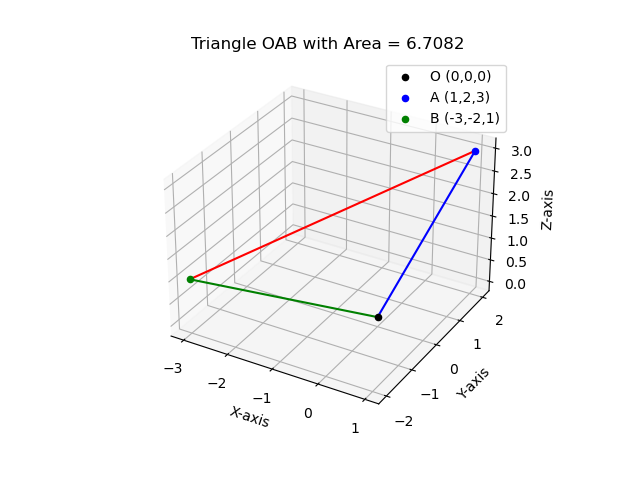
\includegraphics[width=1\linewidth]{Figs/Figure_5.png}
    \caption{}
    \label{fig:fig1}
\end{figure}

\end{document}